\documentclass{beamer}
\usetheme{Madrid}
\usecolortheme{default}

% Packages
\usepackage[utf8]{inputenc}
\usepackage{graphicx}
\usepackage{tikz}
\usetikzlibrary{shapes, arrows, positioning, er}

% Title page information
\title{Entity Relationship Data Model}
\subtitle{Attributes, Constraints, and Database Design}
\author{Nafiul Islam}

\date{\today}

\begin{document}

% Title slide
\begin{frame}
    \titlepage
\end{frame}

% Table of contents
\begin{frame}{Outline}
    \tableofcontents
\end{frame}

% Section 1
\section{Introduction to ER Model}

\begin{frame}{What is the ER Model?}
    \begin{definition}
        The \textbf{Entity-Relationship (ER) Model} is a high-level conceptual data model that represents the data structure of a database in terms of entities, attributes, and relationships.
    \end{definition}
    
    \vspace{0.5cm}
    
    \begin{block}{Purpose of ER Model}
        \begin{itemize}
            \item Provides a visual representation of database structure
            \item Facilitates communication between stakeholders
            \item Serves as a blueprint for database implementation
            \item Identifies entities and their relationships
        \end{itemize}
    \end{block}
\end{frame}

\begin{frame}{History and Importance}
    \textbf{Historical Background:}
    \begin{itemize}
        \item Developed by Peter Chen in 1976
        \item Became a standard for database design
        \item Foundation for modern database modeling
    \end{itemize}
    
    \vspace{0.5cm}
    
    \textbf{Why ER Model is Important:}
    \begin{itemize}
        \item Simplifies complex database structures
        \item Platform-independent design approach
        \item Easy to understand and modify
        \item Reduces development time and errors
        \item Essential for DBMS implementation
    \end{itemize}
\end{frame}

\begin{frame}{Components of ER Model}
    \begin{columns}
        \column{0.5\textwidth}
        \textbf{Main Components:}
        \begin{enumerate}
            \item \textbf{Entities}
            \item \textbf{Attributes}
            \item \textbf{Relationships}
        \end{enumerate}
        
        \column{0.5\textwidth}
        \textbf{ER Diagram Symbols:}
        \begin{itemize}
            \item Rectangle: Entity
            \item Ellipse: Attribute
            \item Diamond: Relationship
            \item Line: Links
        \end{itemize}
    \end{columns}
    
    \vspace{0.5cm}
    
    \begin{alertblock}{Note}
        ER diagrams provide a graphical representation that translates directly to database tables.
    \end{alertblock}
\end{frame}

% Section 2
\section{Entities}

\begin{frame}{Understanding Entities}
    \begin{definition}
        An \textbf{entity} is a real-world object or concept that can be distinctly identified and about which data can be stored in the database.
    \end{definition}
    
    \vspace{0.5cm}
    
    \textbf{Examples of Entities:}
    \begin{itemize}
        \item \textbf{Person:} Student, Employee, Customer
        \item \textbf{Place:} City, University, Branch
        \item \textbf{Object:} Book, Product, Vehicle
        \item \textbf{Event:} Course, Order, Transaction
        \item \textbf{Concept:} Account, Department, Project
    \end{itemize}
\end{frame}

\begin{frame}{Types of Entities}
    \textbf{1. Strong Entity}
    \begin{itemize}
        \item Has its own primary key
        \item Exists independently
        \item Represented by single rectangle
        \item Example: Student, Employee
    \end{itemize}
    
    \vspace{0.3cm}
    
    \textbf{2. Weak Entity}
    \begin{itemize}
        \item Cannot be uniquely identified by its own attributes
        \item Depends on a strong entity (owner entity)
        \item Represented by double rectangle
        \item Example: Dependent (depends on Employee)
    \end{itemize}
\end{frame}

\begin{frame}{Entity Sets}
    \begin{block}{Entity Set}
        A collection of entities of the same type that share the same properties or attributes.
    \end{block}
    
    \vspace{0.5cm}
    
    \begin{example}
        \textbf{Entity Set: STUDENT}
        
        \vspace{0.3cm}
        
        \begin{tabular}{|c|c|c|}
            \hline
            \textbf{Student\_ID} & \textbf{Name} & \textbf{Major} \\
            \hline
            0152430070 & Mainul Islam & Data Science \\
            \hline
            0112410071 & Ahmed Khan & CS \\
            \hline
            0152410002 & Sara Ali & Data Science \\
            \hline
        \end{tabular}
        
        \vspace{0.3cm}
        
        Each row is an \textbf{entity instance}.
    \end{example}
\end{frame}

% Section 3
\section{Attributes}

\begin{frame}{What are Attributes?}
    \begin{definition}
        An \textbf{attribute} is a property or characteristic that describes an entity. Each entity has a set of attributes that define its properties.
    \end{definition}
    
    \vspace{0.5cm}
    
    \begin{exampleblock}{Example: Student Entity}
        Attributes might include:
        \begin{itemize}
            \item Student\_ID
            \item Name
            \item Date\_of\_Birth
            \item Email
            \item Major
            \item GPA
        \end{itemize}
    \end{exampleblock}
\end{frame}

\begin{frame}{Types of Attributes (Part 1)}
    \textbf{1. Simple vs Composite Attributes}
    
    \begin{itemize}
        \item \textbf{Simple (Atomic):} Cannot be divided further
        \begin{itemize}
            \item Example: Age, Gender, Student\_ID
        \end{itemize}
        \item \textbf{Composite:} Can be divided into smaller sub-parts
        \begin{itemize}
            \item Example: Name → (First\_Name, Middle\_Name, Last\_Name)
            \item Example: Address → (Street, City, State, ZIP)
        \end{itemize}
    \end{itemize}
    
    \vspace{0.5cm}
    
    \textbf{2. Single-valued vs Multi-valued Attributes}
    
    \begin{itemize}
        \item \textbf{Single-valued:} One value per entity
        \begin{itemize}
            \item Example: Date\_of\_Birth, Student\_ID
        \end{itemize}
        \item \textbf{Multi-valued:} Multiple values allowed
        \begin{itemize}
            \item Example: Phone\_Numbers, Email\_Addresses
            \item Represented by double ellipse
        \end{itemize}
    \end{itemize}
\end{frame}

\begin{frame}{Types of Attributes (Part 2)}
    \textbf{3. Stored vs Derived Attributes}
    
    \begin{itemize}
        \item \textbf{Stored:} Physically stored in database
        \begin{itemize}
            \item Example: Date\_of\_Birth, Salary
        \end{itemize}
        \item \textbf{Derived:} Calculated from other attributes
        \begin{itemize}
            \item Example: Age (from Date\_of\_Birth)
            \item Example: Total\_Price (from Quantity × Unit\_Price)
            \item Represented by dashed ellipse
        \end{itemize}
    \end{itemize}
    
    \vspace{0.5cm}
    
    \textbf{4. NULL Attributes}
    
    \begin{itemize}
        \item Attributes that may not have a value
        \item Can be \textbf{applicable} (value exists but unknown)
        \item Can be \textbf{not applicable} (attribute doesn't apply)
        \item Example: Middle\_Name (some people don't have one)
    \end{itemize}
\end{frame}

\begin{frame}{Key Attributes}
    \begin{definition}
        A \textbf{key attribute} uniquely identifies each entity in an entity set.
    \end{definition}
    
    \vspace{0.3cm}
    
    \textbf{Types of Keys:}
    
    \begin{enumerate}
        \item \textbf{Super Key:} Any set of attributes that uniquely identifies an entity
        \item \textbf{Candidate Key:} Minimal super key (no redundant attributes)
        \item \textbf{Primary Key:} Chosen candidate key for identification
        \begin{itemize}
            \item Underlined in ER diagrams
            \item Cannot be NULL
        \end{itemize}
        \item \textbf{Composite Key:} Primary key with multiple attributes
        \item \textbf{Foreign Key:} References primary key of another entity
    \end{enumerate}
\end{frame}

\begin{frame}{Attribute Example Visualization}
    \begin{center}
        \textbf{Student Entity with Attributes}
    \end{center}
    
    \vspace{0.3cm}
    
    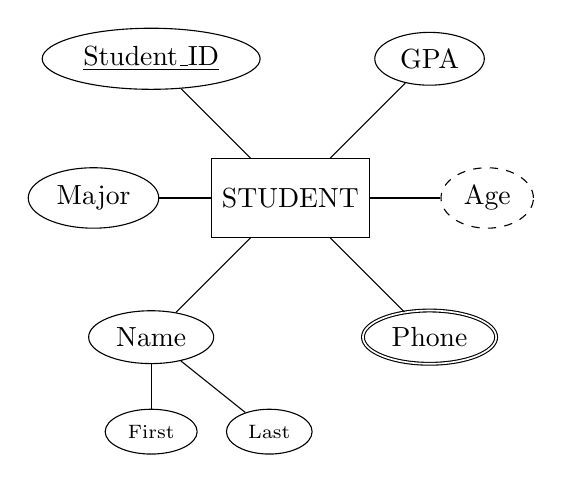
\begin{tikzpicture}[node distance=2cm]
        % Entity
        \node[rectangle, draw, minimum width=2cm, minimum height=1cm] (student) {STUDENT};
        
        % Simple attributes
        \node[ellipse, draw, above left of=student, node distance=2.5cm] (id) {\underline{Student\_ID}};
        \node[ellipse, draw, above right of=student, node distance=2.5cm] (gpa) {GPA};
        \node[ellipse, draw, left of=student, node distance=2.5cm] (major) {Major};
        
        % Composite attribute
        \node[ellipse, draw, below left of=student, node distance=2.5cm] (name) {Name};
        \node[ellipse, draw, below of=name, node distance=1.2cm, font=\scriptsize] (fname) {First};
        \node[ellipse, draw, right of=fname, node distance=1.5cm, font=\scriptsize] (lname) {Last};
        
        % Multi-valued attribute
        \node[ellipse, draw, double, below right of=student, node distance=2.5cm] (phone) {Phone};
        
        % Derived attribute
        \node[ellipse, draw, dashed, right of=student, node distance=2.5cm] (age) {Age};
        
        % Connections
        \draw (id) -- (student);
        \draw (gpa) -- (student);
        \draw (major) -- (student);
        \draw (name) -- (student);
        \draw (phone) -- (student);
        \draw (age) -- (student);
        \draw (name) -- (fname);
        \draw (name) -- (lname);
    \end{tikzpicture}
\end{frame}

% Section 4
\section{Relationships}

\begin{frame}{Understanding Relationships}
    \begin{definition}
        A \textbf{relationship} is an association between two or more entities that represents a meaningful connection in the real world.
    \end{definition}
    
    \vspace{0.5cm}
    
    \begin{exampleblock}{Examples}
        \begin{itemize}
            \item Student \textbf{ENROLLS IN} Course
            \item Employee \textbf{WORKS FOR} Department
            \item Author \textbf{WRITES} Book
            \item Customer \textbf{PLACES} Order
        \end{itemize}
    \end{exampleblock}
    
    \vspace{0.3cm}
    
    \begin{block}{Relationship Set}
        A collection of similar relationships between entity sets.
    \end{block}
\end{frame}

\begin{frame}{Degree of Relationships}
    \textbf{Classification by Number of Participating Entities:}
    
    \begin{enumerate}
        \item \textbf{Unary (Recursive):} Single entity type
        \begin{itemize}
            \item Example: Employee SUPERVISES Employee
            \item Example: Person MARRIED\_TO Person
        \end{itemize}
        
        \vspace{0.3cm}
        
        \item \textbf{Binary:} Two entity types (most common)
        \begin{itemize}
            \item Example: Student ENROLLS Course
            \item Example: Employee WORKS Department
        \end{itemize}
        
        \vspace{0.3cm}
        
        \item \textbf{Ternary:} Three entity types
        \begin{itemize}
            \item Example: Supplier SUPPLIES Part TO Project
            \item Example: Doctor TREATS Patient WITH Medicine
        \end{itemize}
    \end{enumerate}
\end{frame}

\begin{frame}{Cardinality Ratios}
    \textbf{Maximum number of relationship instances an entity can participate in:}
    
    \vspace{0.3cm}
    
    \textbf{1. One-to-One (1:1)}
    \begin{itemize}
        \item Each entity in A relates to at most one entity in B, and vice versa
        \item Example: Person HAS Passport
    \end{itemize}
    
    \textbf{2. One-to-Many (1:N)}
    \begin{itemize}
        \item Entity in A relates to many entities in B
        \item Entity in B relates to at most one entity in A
        \item Example: Department HAS Employees
    \end{itemize}
    
    \textbf{3. Many-to-One (N:1)}
    \begin{itemize}
        \item Reverse of one-to-many
        \item Example: Employees WORK\_IN Department
    \end{itemize}
    
    \textbf{4. Many-to-Many (M:N)}
    \begin{itemize}
        \item Entities in both sets can relate to multiple entities
        \item Example: Students ENROLL Courses
    \end{itemize}
\end{frame}

\begin{frame}{Participation Constraints}
    \textbf{Specifies whether entity existence depends on relationship:}
    
    \vspace{0.5cm}
    
    \textbf{1. Total Participation (Mandatory)}
    \begin{itemize}
        \item Every entity must participate in the relationship
        \item Represented by double line
        \item Example: Every Employee MUST WORK\_IN a Department
    \end{itemize}
    
    \vspace{0.5cm}
    
    \textbf{2. Partial Participation (Optional)}
    \begin{itemize}
        \item Some entities may not participate
        \item Represented by single line
        \item Example: Not every Employee MANAGES a Department
    \end{itemize}
\end{frame}

\begin{frame}{Relationship Attributes}
    \begin{block}{Key Concept}
        Relationships can also have attributes that describe properties of the relationship itself, not the participating entities.
    \end{block}
    
    \vspace{0.5cm}
    
    \begin{example}
        \textbf{Relationship: Student ENROLLS Course}
        
        \vspace{0.2cm}
        
        Relationship Attributes:
        \begin{itemize}
            \item \textbf{Enrollment\_Date:} When student enrolled
            \item \textbf{Grade:} Grade received in the course
            \item \textbf{Semester:} Which semester enrolled
        \end{itemize}
        
        \vspace{0.2cm}
        
        These attributes belong to the relationship, not to Student or Course individually.
    \end{example}
\end{frame}

\begin{frame}{ER Diagram Example}
    \begin{center}
        \textbf{Student - Course Relationship}
    \end{center}
    
    \vspace{0.5cm}
    
    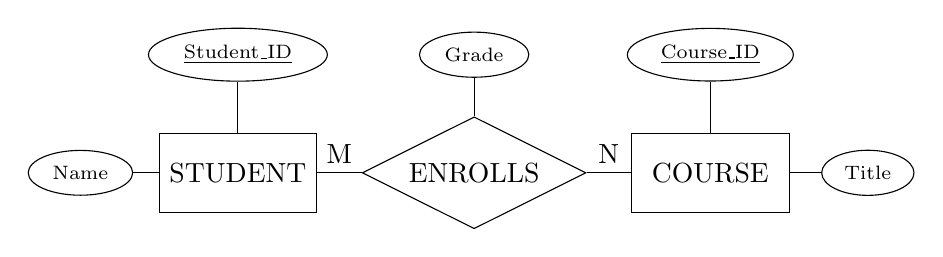
\begin{tikzpicture}[node distance=3cm]
        % Entities
        \node[rectangle, draw, minimum width=2cm, minimum height=1cm] (student) {STUDENT};
        \node[rectangle, draw, minimum width=2cm, minimum height=1cm, right of=student, node distance=6cm] (course) {COURSE};
        
        % Relationship
        \node[diamond, draw, aspect=2, minimum width=2cm, right of=student, node distance=3cm] (enrolls) {ENROLLS};
        
        % Attributes for Student
        \node[ellipse, draw, above of=student, node distance=1.5cm, font=\scriptsize] (sid) {\underline{Student\_ID}};
        \node[ellipse, draw, left of=student, node distance=2cm, font=\scriptsize] (sname) {Name};
        
        % Attributes for Course
        \node[ellipse, draw, above of=course, node distance=1.5cm, font=\scriptsize] (cid) {\underline{Course\_ID}};
        \node[ellipse, draw, right of=course, node distance=2cm, font=\scriptsize] (ctitle) {Title};
        
        % Relationship attribute
        \node[ellipse, draw, above of=enrolls, node distance=1.5cm, font=\scriptsize] (grade) {Grade};
        
        % Connections
        \draw (student) -- node[above] {M} (enrolls);
        \draw (enrolls) -- node[above] {N} (course);
        \draw (sid) -- (student);
        \draw (sname) -- (student);
        \draw (cid) -- (course);
        \draw (ctitle) -- (course);
        \draw (grade) -- (enrolls);
    \end{tikzpicture}
    
    \vspace{0.3cm}
    
    \begin{alertblock}{Cardinality}
        M:N relationship - Many students can enroll in many courses
    \end{alertblock}
\end{frame}

% Section 5
\section{Constraints in ER Model}

\begin{frame}{Introduction to Constraints}
    \begin{definition}
        \textbf{Constraints} are rules that restrict the data that can be stored in the database, ensuring data integrity and consistency.
    \end{definition}
    
    \vspace{0.5cm}
    
    \textbf{Why Constraints are Important:}
    \begin{itemize}
        \item Maintain data accuracy and consistency
        \item Prevent invalid data entry
        \item Enforce business rules
        \item Ensure referential integrity
        \item Support data quality
    \end{itemize}
\end{frame}

\begin{frame}{Types of Constraints}
    \textbf{Main Categories of Constraints:}
    
    \begin{enumerate}
        \item \textbf{Key Constraints}
        \item \textbf{Participation Constraints}
        \item \textbf{Cardinality Constraints}
        \item \textbf{Domain Constraints}
        \item \textbf{Integrity Constraints}
    \end{enumerate}
    
    \vspace{0.5cm}
    
    \begin{block}{Note}
        Constraints are specified during database design and enforced by the DBMS during operations.
    \end{block}
\end{frame}

\begin{frame}{Key Constraints}
    \textbf{Ensure Unique Identification:}
    
    \vspace{0.3cm}
    
    \textbf{1. Primary Key Constraint}
    \begin{itemize}
        \item Each entity must have a unique identifier
        \item Cannot contain NULL values
        \item Only one primary key per entity
        \item Example: Student\_ID for STUDENT entity
    \end{itemize}
    
    \vspace{0.3cm}
    
    \textbf{2. Unique Constraint}
    \begin{itemize}
        \item Ensures attribute values are unique
        \item Can contain NULL values
        \item Multiple unique constraints allowed
        \item Example: Email address must be unique
    \end{itemize}
\end{frame}

\begin{frame}{Participation Constraints (Revisited)}
    \textbf{Define Mandatory vs Optional Relationships:}
    
    \vspace{0.5cm}
    
    \begin{columns}
        \column{0.5\textwidth}
        \textbf{Total Participation:}
        \begin{itemize}
            \item Minimum cardinality: 1
            \item Every entity must participate
            \item Example: Employee must belong to Department
            \item Notation: Double line or (1,N)
        \end{itemize}
        
        \column{0.5\textwidth}
        \textbf{Partial Participation:}
        \begin{itemize}
            \item Minimum cardinality: 0
            \item Participation is optional
            \item Example: Employee may manage Department
            \item Notation: Single line or (0,N)
        \end{itemize}
    \end{columns}
\end{frame}

\begin{frame}{Cardinality Constraints}
    \textbf{Specify Number of Relationship Instances:}
    
    \vspace{0.3cm}
    
    \begin{block}{Min-Max Notation (m,n)}
        \begin{itemize}
            \item \textbf{m:} Minimum participation (0 = optional, 1 = mandatory)
            \item \textbf{n:} Maximum participation (1, N, M for many)
        \end{itemize}
    \end{block}
    
    \vspace{0.3cm}
    
    \begin{example}
        \textbf{Employee WORKS\_IN Department}
        
        \vspace{0.2cm}
        
        \begin{itemize}
            \item Employee side: (1,1) - Each employee works in exactly one department
            \item Department side: (0,N) - Department can have zero or many employees
        \end{itemize}
    \end{example}
\end{frame}

\begin{frame}{Domain Constraints}
    \textbf{Restrict Allowable Attribute Values:}
    
    \vspace{0.3cm}
    
    \textbf{Types of Domain Constraints:}
    
    \begin{enumerate}
        \item \textbf{Data Type:} Integer, String, Date, etc.
        \begin{itemize}
            \item Example: Age must be Integer
        \end{itemize}
        
        \item \textbf{Range:} Minimum and maximum values
        \begin{itemize}
            \item Example: Age between 18 and 100
        \end{itemize}
        
        \item \textbf{Format:} Pattern for values
        \begin{itemize}
            \item Example: Email must contain '@'
        \end{itemize}
        
        \item \textbf{Enumerated Values:} Fixed set of options
        \begin{itemize}
            \item Example: Gender in \{'Male', 'Female', 'Other'\}
        \end{itemize}
    \end{enumerate}
\end{frame}

\begin{frame}{Integrity Constraints}
    \textbf{1. Entity Integrity Constraint}
    \begin{itemize}
        \item Primary key cannot be NULL
        \item Ensures each entity is uniquely identifiable
    \end{itemize}
    
    \vspace{0.3cm}
    
    \textbf{2. Referential Integrity Constraint}
    \begin{itemize}
        \item Foreign key must reference existing primary key
        \item Maintains consistency across tables
        \item Example: Student's Department\_ID must exist in DEPARTMENT table
    \end{itemize}
    
    \vspace{0.3cm}
    
    \textbf{3. Semantic Integrity Constraint}
    \begin{itemize}
        \item Business rules specific to application
        \item Example: Enrollment\_Date must be before Graduation\_Date
        \item Example: Employee Salary must be positive
    \end{itemize}
\end{frame}

\begin{frame}{Additional Constraints}
    \textbf{NOT NULL Constraint}
    \begin{itemize}
        \item Attribute must have a value
        \item Example: Student Name cannot be NULL
    \end{itemize}
    
    \vspace{0.3cm}
    
    \textbf{CHECK Constraint}
    \begin{itemize}
        \item Validates data against a condition
        \item Example: GPA CHECK (GPA >= 0.0 AND GPA <= 4.0)
    \end{itemize}
    
    \vspace{0.3cm}
    
    \textbf{DEFAULT Constraint}
    \begin{itemize}
        \item Provides default value if none specified
        \item Example: Country DEFAULT 'Bangladesh'
    \end{itemize}
\end{frame}

% Section 6
\section{Extended ER Features}

\begin{frame}{Specialization and Generalization}
    \textbf{Specialization (Top-Down):}
    \begin{itemize}
        \item Process of defining subclasses from a superclass
        \item Subclasses inherit attributes from superclass
        \item Example: PERSON → STUDENT, EMPLOYEE
    \end{itemize}
    
    \vspace{0.3cm}
    
    \textbf{Generalization (Bottom-Up):}
    \begin{itemize}
        \item Process of combining similar entities into a superclass
        \item Identifies common attributes
        \item Example: CAR, TRUCK, MOTORCYCLE → VEHICLE
    \end{itemize}
    
    \vspace{0.3cm}
    
    \begin{alertblock}{IS-A Relationship}
        Represented by triangle in ER diagrams. Student IS-A Person.
    \end{alertblock}
\end{frame}

\begin{frame}{Aggregation}
    \begin{definition}
        \textbf{Aggregation} treats a relationship as a higher-level entity, allowing relationships to participate in other relationships.
    \end{definition}
    
    \vspace{0.5cm}
    
    \begin{example}
        \textbf{Scenario:} Projects use employees as consultants
        
        \vspace{0.2cm}
        
        \begin{enumerate}
            \item Employee WORKS\_ON Project (basic relationship)
            \item This work assignment is MONITORED\_BY Manager
            \item (Employee, WORKS\_ON, Project) becomes an aggregated entity
            \item Aggregation participates in MONITORED\_BY relationship
        \end{enumerate}
    \end{example}
    
    \vspace{0.3cm}
    
    \begin{block}{Representation}
        Shown by enclosing relationship in a rectangle (box).
    \end{block}
\end{frame}

% Section 7
\section{ER to Relational Mapping}

\begin{frame}{Converting ER Model to Tables}
    \textbf{Why Mapping is Needed:}
    \begin{itemize}
        \item ER model is conceptual (design phase)
        \item Relational model is logical (implementation)
        \item DBMS works with tables, not ER diagrams
    \end{itemize}
    
    \vspace{0.5cm}
    
    \textbf{Basic Mapping Rules:}
    \begin{enumerate}
        \item Entities → Tables
        \item Attributes → Columns
        \item Primary Keys → Primary Key Columns
        \item Relationships → Foreign Keys or Tables
    \end{enumerate}
\end{frame}

\begin{frame}{Mapping Strong Entities}
    \textbf{Rule:} Each strong entity becomes a table
    
    \vspace{0.3cm}
    
    \begin{example}
        \textbf{STUDENT Entity with attributes:} \\
        Student\_ID (PK), Name, Email, Major
        
        \vspace{0.3cm}
        
        \textbf{Becomes Table:}
        
        \vspace{0.2cm}
        
        \begin{tabular}{|c|c|c|c|}
            \hline
            \textbf{Student\_ID} & \textbf{Name} & \textbf{Email} & \textbf{Major} \\
            \hline
            0152410070 & Nafiul Islam & nafiul@uiu.ac.bd & Data Science \\
            \hline
            ... & ... & ... & ... \\
            \hline
        \end{tabular}
        
        \vspace{0.3cm}
        
        Student\_ID becomes PRIMARY KEY
    \end{example}
\end{frame}

\begin{frame}{Mapping Weak Entities}
    \textbf{Rule:} Create table with partial key + foreign key to owner
    
    \vspace{0.3cm}
    
    \begin{example}
        \textbf{Weak Entity:} DEPENDENT \\
        Partial Key: Dependent\_Name \\
        Owner Entity: EMPLOYEE (Employee\_ID)
        
        \vspace{0.3cm}
        
        \textbf{DEPENDENT Table:}
        
        \vspace{0.2cm}
        
        \begin{tabular}{|c|c|c|}
            \hline
            \textbf{Employee\_ID (FK)} & \textbf{Dependent\_Name} & \textbf{Relationship} \\
            \hline
            E001 & Ahmed & Son \\
            \hline
            E001 & Fatima & Daughter \\
            \hline
            E002 & Ali & Son \\
            \hline
        \end{tabular}
        
        \vspace{0.3cm}
        
        Composite Primary Key: (Employee\_ID, Dependent\_Name)
    \end{example}
\end{frame}

\begin{frame}{Mapping Relationships}
    \textbf{1:1 Relationship:} Add foreign key to either table (prefer total participation side)
    
    \vspace{0.2cm}
    
    \textbf{1:N Relationship:} Add foreign key to N-side table
    \begin{itemize}
        \item Example: Department (1) — EMPLOYS — (N) Employee
        \item Add Department\_ID as FK in EMPLOYEE table
    \end{itemize}
    
    \vspace{0.2cm}
    
    \textbf{M:N Relationship:} Create new table with FKs from both entities
    \begin{itemize}
        \item Example: Student (M) — ENROLLS — (N) Course
        \item Create ENROLLMENT table:
        \item Columns: Student\_ID (FK), Course\_ID (FK), Grade
        \item Composite PK: (Student\_ID, Course\_ID)
    \end{itemize}
\end{frame}

\begin{frame}{Mapping Multi-valued Attributes}
    \textbf{Rule:} Create a separate table
    
    \vspace{0.3cm}
    
    \begin{example}
        \textbf{Entity:} EMPLOYEE with multi-valued attribute Phone\_Numbers
        
        \vspace{0.3cm}
        
        \textbf{Create EMPLOYEE\_PHONE Table:}
        
        \vspace{0.2cm}
        
        \begin{tabular}{|c|c|}
            \hline
            \textbf{Employee\_ID (FK)} & \textbf{Phone\_Number} \\
            \hline
            E001 & +880-1711-123456 \\
            \hline
            E001 & +880-2-9876543 \\
            \hline
            E002 & +880-1812-654321 \\
            \hline
        \end{tabular}
        
        \vspace{0.3cm}
        
        Primary Key: (Employee\_ID, Phone\_Number)
    \end{example}
\end{frame}

\begin{frame}{Complete Mapping Example}
    \textbf{ER Diagram: University Database}
    
    \vspace{0.2cm}
    
    \textbf{Entities:} STUDENT, COURSE, INSTRUCTOR
    
    \textbf{Relationships:} 
    \begin{itemize}
        \item STUDENT (M) — ENROLLS — (N) COURSE
        \item INSTRUCTOR (1) — TEACHES — (N) COURSE
    \end{itemize}
    
    \vspace{0.3cm}
    
    \textbf{Resulting Tables:}
    \begin{enumerate}
        \item \textbf{STUDENT} (Student\_ID, Name, Email, Major)
        \item \textbf{COURSE} (Course\_ID, Title, Credits, Instructor\_ID)
        \item \textbf{INSTRUCTOR} (Instructor\_ID, Name, Department)
        \item \textbf{ENROLLMENT} (Student\_ID, Course\_ID, Grade, Semester)
    \end{enumerate}
\end{frame}

% Section 8
\section{Practical Applications}

\begin{frame}{Real-World ER Modeling Example}
    \textbf{Case Study: Online Shopping System}
    
    \vspace{0.3cm}
    
    \textbf{Key Entities:}
    \begin{itemize}
        \item CUSTOMER
        \item PRODUCT
        \item ORDER
        \item PAYMENT
    \end{itemize}
    
    \vspace{0.3cm}
    
    \textbf{Relationships:}
    \begin{itemize}
        \item Customer PLACES Order (1:N)
        \item Order CONTAINS Product (M:N)
        \item Order HAS Payment (1:1)
    \end{itemize}
\end{frame}

\begin{frame}{Design Best Practices}
    \textbf{Guidelines for Good ER Design:}
    
    \begin{enumerate}
        \item \textbf{Completeness:} Capture all requirements
        \item \textbf{Correctness:} Model real-world accurately
        \item \textbf{Minimality:} Avoid redundancy
        \item \textbf{Clarity:} Use meaningful names
        \item \textbf{Normalization:} Reduce data duplication
        \item \textbf{Documentation:} Explain design decisions
    \end{enumerate}
    
    \vspace{0.3cm}
    
    \begin{alertblock}{Common Mistakes to Avoid}
        \begin{itemize}
            \item Using entities as attributes
            \item Redundant relationships
            \item Incorrect cardinality
            \item Missing constraints
        \end{itemize}
    \end{alertblock}
\end{frame}

\begin{frame}{ER Model in Data Science}
    \textbf{Why Data Scientists Need ER Modeling:}
    
    \begin{itemize}
        \item \textbf{Data Understanding:} Understand structure before analysis
        \item \textbf{Data Integration:} Combine data from multiple sources
        \item \textbf{Feature Engineering:} Identify relationships for features
        \item \textbf{Data Warehousing:} Design analytical databases
        \item \textbf{Big Data:} Model NoSQL and distributed databases
    \end{itemize}
    
    \vspace{0.3cm}
    
    \begin{exampleblock}{Application}
        In machine learning projects, ER models help identify:
        \begin{itemize}
            \item Which tables to join for training data
            \item Relationship features (e.g., customer-product interactions)
            \item Data lineage and dependencies
        \end{itemize}
    \end{exampleblock}
\end{frame}

% Section 9
\section{Learning Outcomes}

\begin{frame}{Key Takeaways}
    \begin{block}{What You Should Now Understand:}
    \end{block}
    
    \begin{itemize}
        \item \checkmark ER Model components: Entities, Attributes, Relationships
        \item \checkmark Different types of attributes and their representations
        \item \checkmark Relationship types and cardinality constraints
        \item \checkmark Various constraints ensuring data integrity
        \item \checkmark Extended ER features: Specialization, Generalization, Aggregation
        \item \checkmark Converting ER diagrams to relational tables
        \item \checkmark Real-world application of ER modeling
        \item \checkmark Importance of proper database design in DBMS
    \end{itemize}
\end{frame}

\begin{frame}{Importance of ER Model in DBMS}
    \textbf{Why ER Model Matters:}
    
    \begin{enumerate}
        \item \textbf{Foundation of Database Design}
        \begin{itemize}
            \item Blueprint for entire database structure
            \item Prevents costly redesigns later
        \end{itemize}
        
        \item \textbf{Communication Tool}
        \begin{itemize}
            \item Bridge between users and developers
            \item Visual representation everyone understands
        \end{itemize}
        
        \item \textbf{Data Integrity}
        \begin{itemize}
            \item Constraints prevent invalid data
            \item Maintains consistency and accuracy
        \end{itemize}
        
        \item \textbf{Efficient Implementation}
        \begin{itemize}
            \item Optimized table structures
            \item Better query performance
        \end{itemize}
    \end{enumerate}
\end{frame}

% Conclusion
\section{Conclusion}

\begin{frame}{Summary}
    \textbf{Topics Covered:}
    
    \begin{itemize}
        \item Introduction to ER Model and its components
        \item Understanding Entities (Strong and Weak)
        \item Comprehensive coverage of Attributes types
        \item Relationships and their classifications
        \item Detailed exploration of Constraints
        \item Extended ER features
        \item ER to Relational mapping techniques
        \item Practical applications and best practices
    \end{itemize}
    
    \vspace{0.5cm}
    
    \begin{center}
        \Large
        \textbf{Questions?}
    \end{center}
\end{frame}

\begin{frame}{Further Learning Resources}
    \textbf{Recommended Reading:}
    
    \begin{itemize}
        \item Fundamentals of Database Systems - Elmasri \& Navathe
        \item Database System Concepts - Silberschatz, Korth, Sudarshan
        \item Database Management Systems - Ramakrishnan \& Gehrke
    \end{itemize}
    
    \vspace{0.3cm}
    
    \textbf{Online Resources:}
    \begin{itemize}
        \item W3Schools Database Tutorial
        \item Oracle Database Documentation
        \item Stanford Database Course (Coursera)
    \end{itemize}
    
    \vspace{0.5cm}
    
    \begin{center}
        \Large
        \textbf{Thank You!}
        
        \vspace{0.5cm}
        
        \normalsize
        Nafiul Islam \\
        ID: 0152410070 \\
        Data Science, UIU
    \end{center}
\end{frame}

\end{document}
